\documentclass[12pt]{article}
\usepackage{color}
\usepackage{tikz}
\usepackage{amssymb}

\begin{document}

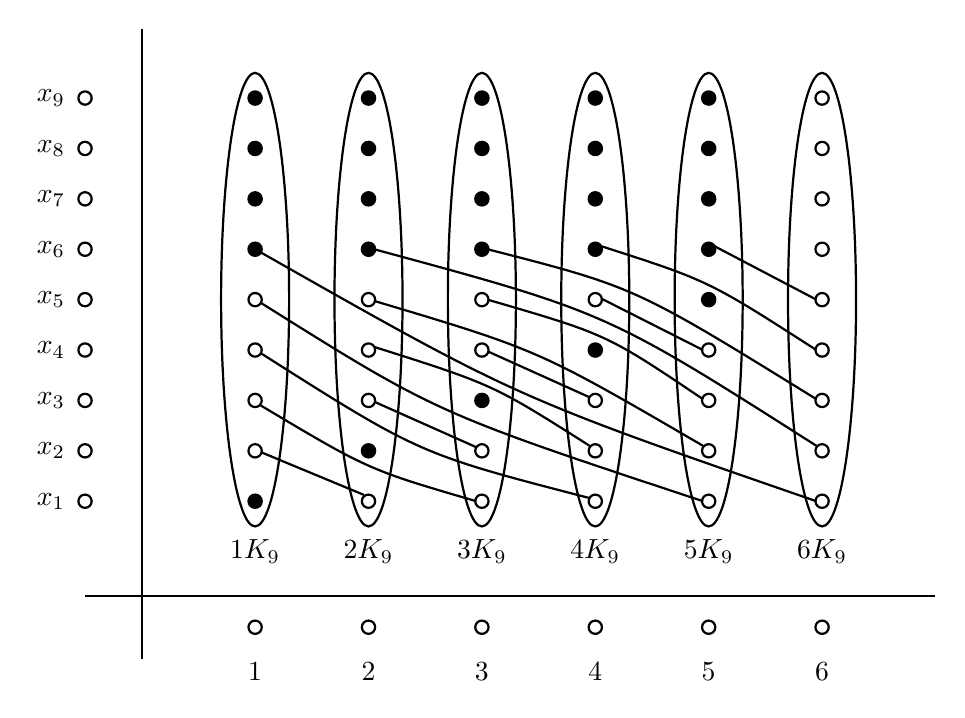
\begin{tikzpicture}[scale=0.8,style=thick,x=1.8cm,y=1cm]
\def\vr{3pt}

\begin{scope}[xshift=0cm, yshift=0cm] % C4 1
\coordinate(x1) at (1,0);
\coordinate(x2) at (2,0);
\coordinate(x3) at (3,0);
\coordinate(x4) at (4,0);
\coordinate(x5) at (5,0);
\coordinate(x6) at (6,0);
\coordinate(u1) at (1,-2);
\coordinate(u2) at (2,-2);
\coordinate(u3) at (3,-2);
\coordinate(u4) at (4,-2);
\coordinate(u5) at (5,-2);
\coordinate(u6) at (6,-2);
\coordinate(y1) at (-0.5,0);
\coordinate(y2) at (-0.5,0.8);
\coordinate(y3) at (-0.5,1.6);
\coordinate(y4) at (-0.5,2.4);
\coordinate(y5) at (-0.5,3.2);
\coordinate(y6) at (-0.5,4.0);
\coordinate(y7) at (-0.5,4.8);
\coordinate(y8) at (-0.5,5.6);
\coordinate(y9) at (-0.5,6.4);

\draw (-0.5,-1.5) -- (7,-1.5);
\draw (0,-2.5) -- (0,7.5);

%  vertices
\draw(x1)[fill=black] circle(\vr);
\draw(x2)[fill=white] circle(\vr);
\draw(x3)[fill=white] circle(\vr);
\draw(x4)[fill=white] circle(\vr);
\draw(x5)[fill=white] circle(\vr);
\draw(x6)[fill=white] circle(\vr);
\draw(u1)[fill=white] circle(\vr);
\draw(u2)[fill=white] circle(\vr);
\draw(u3)[fill=white] circle(\vr);
\draw(u4)[fill=white] circle(\vr);
\draw(u5)[fill=white] circle(\vr);
\draw(u6)[fill=white] circle(\vr);
\draw(y1)[fill=white] circle(\vr);
\draw(y2)[fill=white] circle(\vr);
\draw(y3)[fill=white] circle(\vr);
\draw(y4)[fill=white] circle(\vr);
\draw(y5)[fill=white] circle(\vr);
\draw(y6)[fill=white] circle(\vr);
\draw(y7)[fill=white] circle(\vr);
\draw(y8)[fill=white] circle(\vr);
\draw(y9)[fill=white] circle(\vr);

\draw (1,3.2) ellipse (0.3 and 3.6);
\node at (1,-0.8) {$1K_9$};
\end{scope}

\begin{scope}[xshift=0cm, yshift=0.8cm] % C4 2
\coordinate(x1) at (1,0);
\coordinate(x2) at (2,0);
\coordinate(x3) at (3,0);
\coordinate(x4) at (4,0);
\coordinate(x5) at (5,0);
\coordinate(x6) at (6,0);
%  vertices
\draw(x1)[fill=white] circle(\vr);
\draw(x2)[fill=black] circle(\vr);
\draw(x3)[fill=white] circle(\vr);
\draw(x4)[fill=white] circle(\vr);
\draw(x5)[fill=white] circle(\vr);
\draw(x6)[fill=white] circle(\vr);

\draw (2,2.4) ellipse (0.3 and 3.6);
\node at (1, -3.5) {$1$};
\node at (2, -3.5) {$2$};
\node at (3, -3.5) {$3$};
\node at (4, -3.5) {$4$};
\node at (5, -3.5) {$5$};
\node at (6, -3.5) {$6$};
\node at (-0.8, -0.8) {$x_1$};
\node at (-0.8, 0) {$x_2$};
\node at (-0.8, 0.8) {$x_3$};
\node at (-0.8, 1.6) {$x_4$};
\node at (-0.8, 2.4) {$x_5$};
\node at (-0.8, 3.2) {$x_6$};
\node at (-0.8, 4.0) {$x_7$};
\node at (-0.8, 4.8) {$x_8$};
\node at (-0.8, 5.6) {$x_9$};
\node at (2,-1.6) {$2K_9$};
\end{scope}

\begin{scope}[xshift=0cm, yshift=1.6cm] % C4 3
\coordinate(x1) at (1,0);
\coordinate(x2) at (2,0);
\coordinate(x3) at (3,0);
\coordinate(x4) at (4,0);
\coordinate(x5) at (5,0);
\coordinate(x6) at (6,0);

%  vertices
\draw(x1)[fill=white] circle(\vr);
\draw(x2)[fill=white] circle(\vr);
\draw(x3)[fill=black] circle(\vr);
\draw(x4)[fill=white] circle(\vr);
\draw(x5)[fill=white] circle(\vr);
\draw(x6)[fill=white] circle(\vr);

\draw (3,1.6) ellipse (0.3 and 3.6);
\node at (3,-2.4) {$3K_9$};
\end{scope}

\begin{scope}[xshift=0cm, yshift=2.4cm] % C4 4
\coordinate(x1) at (1,0);
\coordinate(x2) at (2,0);
\coordinate(x3) at (3,0);
\coordinate(x4) at (4,0);
\coordinate(x5) at (5,0);
\coordinate(x6) at (6,0);
%  vertices
\draw(x1)[fill=white] circle(\vr);
\draw(x2)[fill=white] circle(\vr);
\draw(x3)[fill=white] circle(\vr);
\draw(x4)[fill=black] circle(\vr);
\draw(x5)[fill=white] circle(\vr);
\draw(x6)[fill=white] circle(\vr);

\draw (4,0.8) ellipse (0.3 and 3.6);
\node at (4,-3.2) {$4K_9$};
\end{scope}

\begin{scope}[xshift=0cm, yshift=3.2cm] % C4 5
\coordinate(x1) at (1,0);
\coordinate(x2) at (2,0);
\coordinate(x3) at (3,0);
\coordinate(x4) at (4,0);
\coordinate(x5) at (5,0);
\coordinate(x6) at (6,0);
%  vertices
\draw(x1)[fill=white] circle(\vr);
\draw(x2)[fill=white] circle(\vr);
\draw(x3)[fill=white] circle(\vr);
\draw(x4)[fill=white] circle(\vr);
\draw(x5)[fill=black] circle(\vr);
\draw(x6)[fill=white] circle(\vr);

\draw (5,0) ellipse (0.3 and 3.6);
\node at (5,-4) {$5K_9$};
\end{scope}

\begin{scope}[xshift=0cm, yshift=4cm] % C4 6
\coordinate(x1) at (1,0);
\coordinate(x2) at (2,0);
\coordinate(x3) at (3,0);
\coordinate(x4) at (4,0);
\coordinate(x5) at (5,0);
\coordinate(x6) at (6,0);
%  vertices
\draw(x1)[fill=black] circle(\vr);
\draw(x2)[fill=black] circle(\vr);
\draw(x3)[fill=black] circle(\vr);
\draw(x4)[fill=black] circle(\vr);
\draw(x5)[fill=black] circle(\vr);
\draw(x6)[fill=white] circle(\vr);

\draw (6,-0.8) ellipse (0.3 and 3.6);
\node at (6,-4.8) {$6K_9$};
\end{scope}

\begin{scope}[xshift=0cm, yshift=4.8cm] % C4 7
\coordinate(x1) at (1,0);
\coordinate(x2) at (2,0);
\coordinate(x3) at (3,0);
\coordinate(x4) at (4,0);
\coordinate(x5) at (5,0);
\coordinate(x6) at (6,0);
%  vertices
\draw(x1)[fill=black] circle(\vr);
\draw(x2)[fill=black] circle(\vr);
\draw(x3)[fill=black] circle(\vr);
\draw(x4)[fill=black] circle(\vr);
\draw(x5)[fill=black] circle(\vr);
\draw(x6)[fill=white] circle(\vr);
\end{scope}


\begin{scope}[xshift=0cm, yshift=5.6cm] % C4 8
\coordinate(x1) at (1,0);
\coordinate(x2) at (2,0);
\coordinate(x3) at (3,0);
\coordinate(x4) at (4,0);
\coordinate(x5) at (5,0);
\coordinate(x6) at (6,0);
%  vertices
\draw(x1)[fill=black] circle(\vr);
\draw(x2)[fill=black] circle(\vr);
\draw(x3)[fill=black] circle(\vr);
\draw(x4)[fill=black] circle(\vr);
\draw(x5)[fill=black] circle(\vr);
\draw(x6)[fill=white] circle(\vr);
\end{scope}

\begin{scope}[xshift=0cm, yshift=6.4cm] % C4 9
\coordinate(x1) at (1,0);
\coordinate(x2) at (2,0);
\coordinate(x3) at (3,0);
\coordinate(x4) at (4,0);
\coordinate(x5) at (5,0);
\coordinate(x6) at (6,0);
%  vertices
\draw(x1)[fill=black] circle(\vr);
\draw(x2)[fill=black] circle(\vr);
\draw(x3)[fill=black] circle(\vr);
\draw(x4)[fill=black] circle(\vr);
\draw(x5)[fill=black] circle(\vr);
\draw(x6)[fill=white] circle(\vr);
\end{scope}

\draw (1.05,0.78) -- (1.96,0.1);
\draw (1.05,1.52) .. controls (2,0.5).. (2.95,0);
\draw (1.05,2.35) .. controls (2.45,0.75).. (3.95,0.05);
\draw (2.05,1.58) -- (2.96,0.85);
\draw (1.05,3.15) .. controls (2.6,1.4).. (4.95,0);
\draw (2.05,2.45) .. controls (3.1,1.85).. (3.95,0.88);
\draw (1.05,3.95) .. controls (3.3,1.65).. (5.95,0);
\draw (3.05,2.38) -- (3.95,1.65);
\draw (2.05,3.18) .. controls (3.5,2.4).. (4.95,0.88);
\draw (3.05,3.2) .. controls (4.1,2.65).. (4.95,1.62);
\draw (2.05,4) .. controls (4.1,3).. (5.95,0.88);
\draw (4.05,3.22) -- (4.95,2.4);
\draw (3.05,4) .. controls (4.35,3.4).. (5.95,1.62);
\draw (4.05,4.05) .. controls (5,3.5).. (5.95,2.4);
\draw (5.05,4.05) -- (5.95,3.2);

\end{tikzpicture}

\end{document}